\begin{frame}\frametitle{Theory. EWK Interactions}
\end{frame}%{Theory. Weak Interactions}

\begin{frame}\frametitle{Theory. Anomalous Gauge Couplings}
\end{frame}%{Theory. Anomalous Gauge Couplings}

\begin{frame}\frametitle{Theory. $W\gamma\rightarrow l\nu\gamma$}
\scriptsize
\begin{figure}[htb]
\begin{center}
\scriptsize
%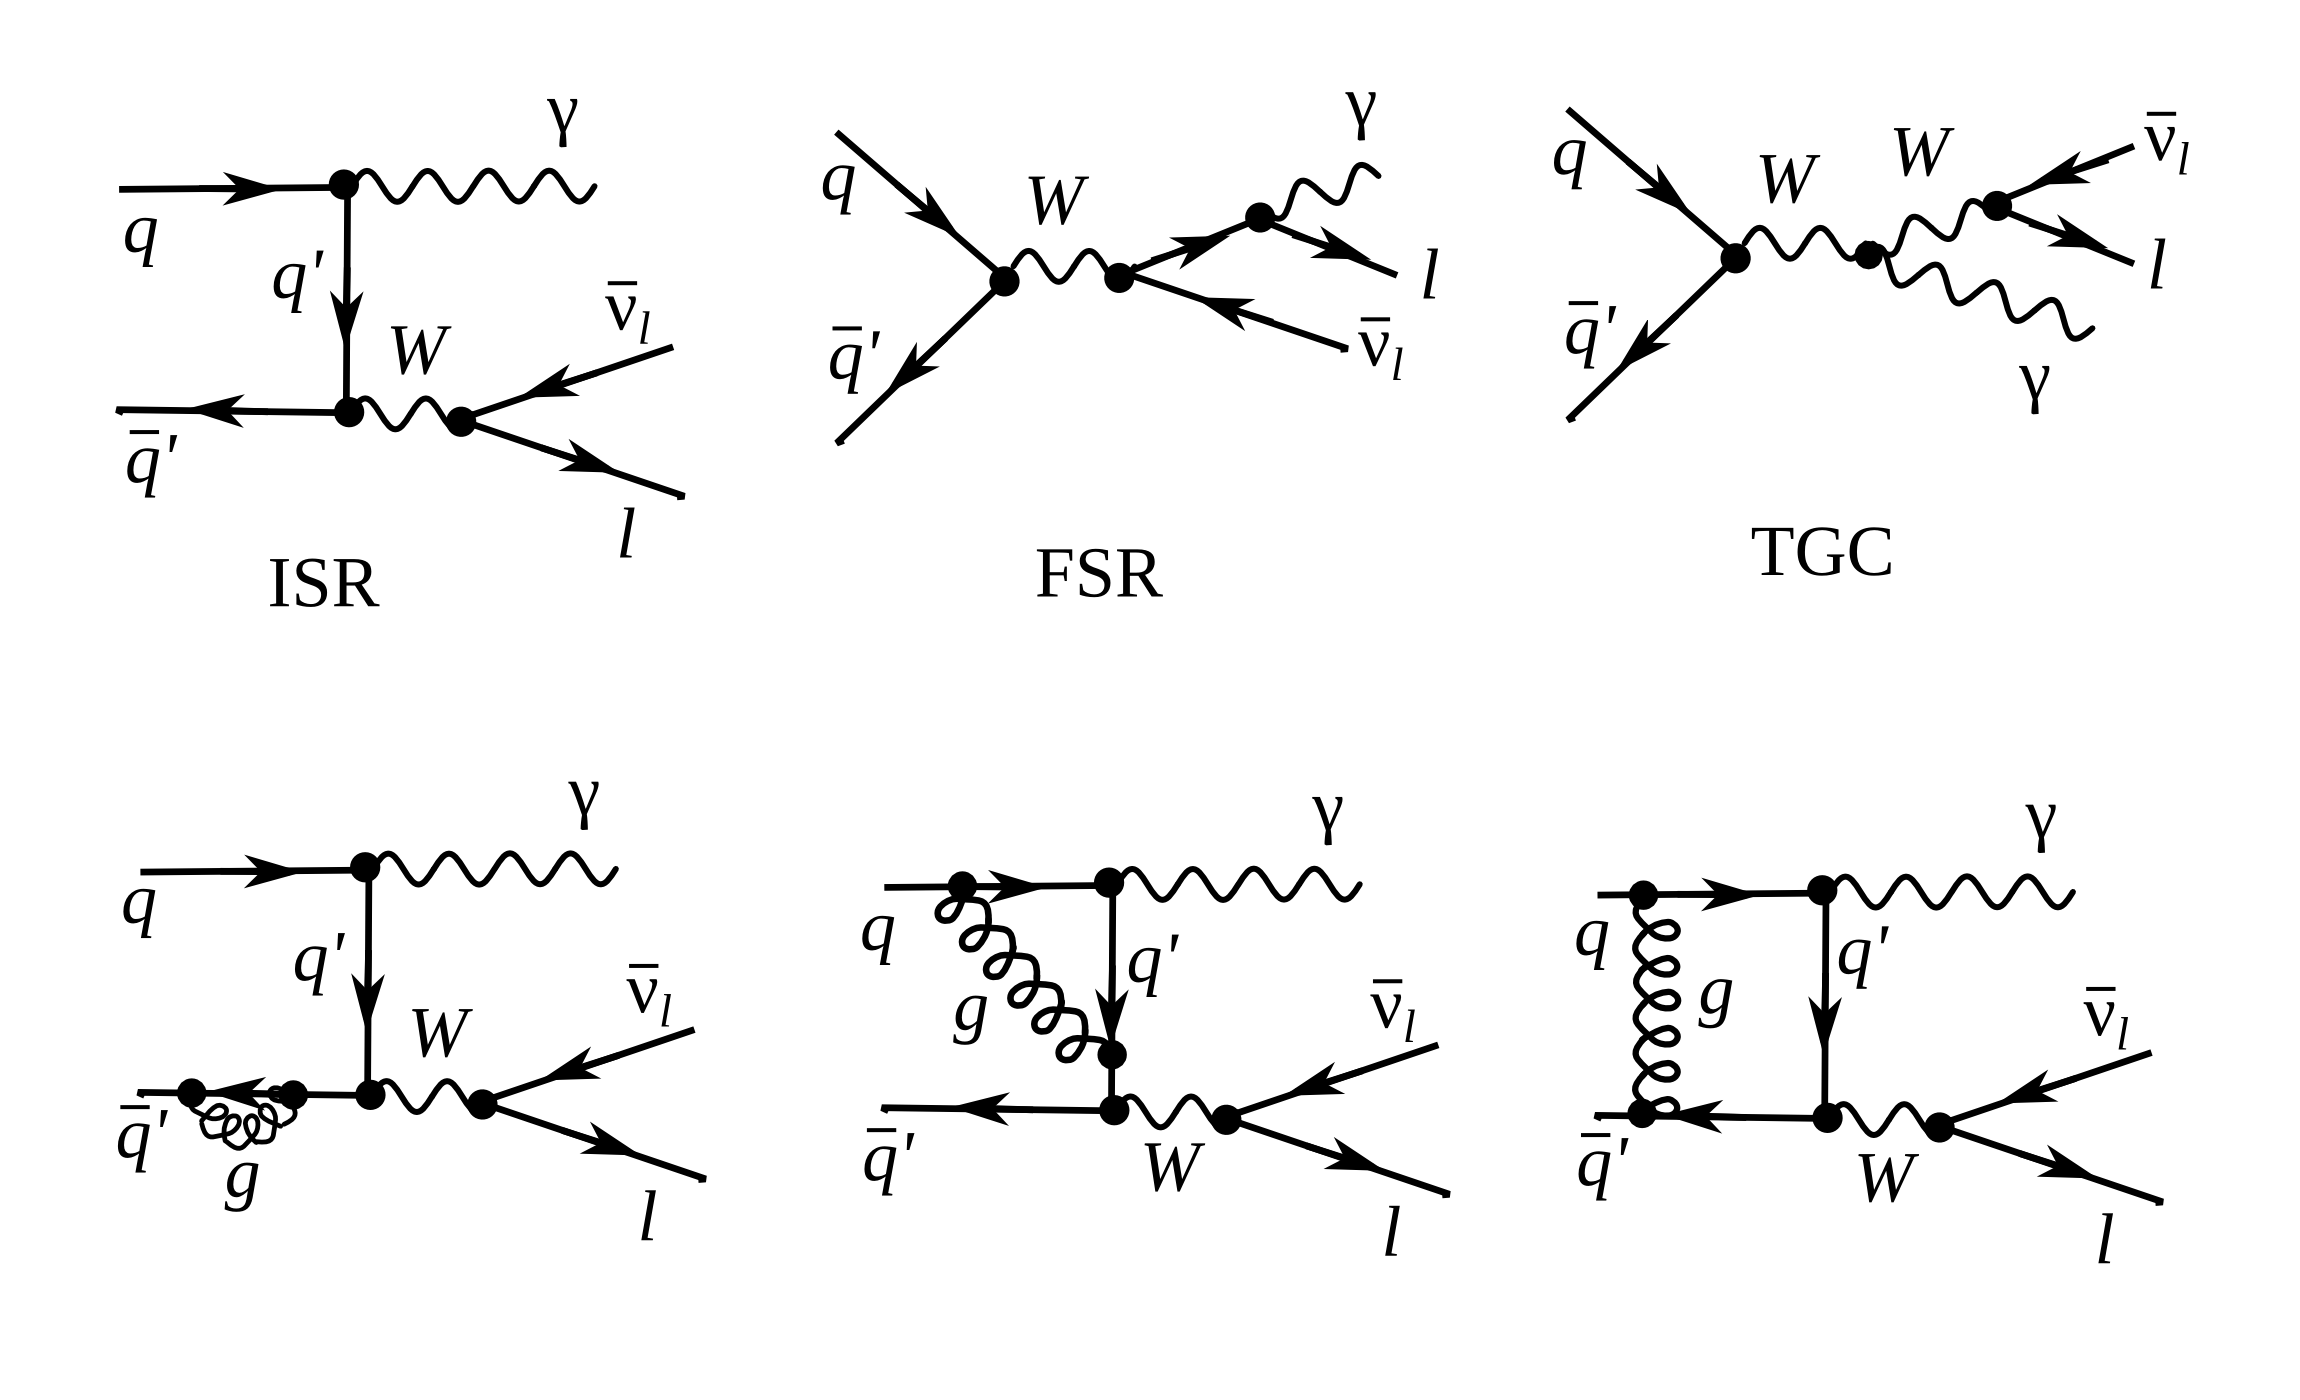
\includegraphics[width=0.95\textwidth]{../figs/WgAbout/feynmWg_LO_NLO.png}
%\caption{\scriptsize{The Feynman diagrams. ISR(x2), FSR, and TGC.}}
\end{center}
\end{figure}
\scriptsize
Process signature:\\
\begin{itemize}
\item prompt, energetic, and isolated muon/electron
\item prompt isolated photon
\item significant missing energy due to neutrino 
\end{itemize}
Goals:\\
\begin{itemize}
\item measure total and differential $\frac{d\sigma}{dp_{T}^{\gamma}}$cross section
%\item set limits on aTGC constants (or detect aTGC)
\end{itemize}
Motivation:\\
\begin{itemize}
\item test Standard Model
%\item provide precise cross section result for measurements where W$\gamma$ is significant background
\end{itemize}
\end{frame}%{Theory. $W\gamma\rightarrow l\nu\gamma$}
